\newpage
\chapter{Samples}
\label{chap:Samples}

\section{Sample 01: Potential handling}

The aim of this series of examples is mainly to show how to handle the creation of variables and factors.

\subsection{Variables creation}

\subsubsection{part 01}

This example creates a tow initial variables $A$ and $B$ with a domain size equal to 2 and places them into a group storing them. Later, it adds variables $C$ and $D$, with the same domain size. Finally, tries to add again $C$, showing the this further addition is correctly refused.

\subsubsection{part 02}

This example considers 3 variables $A$, $B$ and $C$ with a domain sizes equal to, respectively, 2,4 and 3, i.e:
\begin{eqnarray}
Dom(A) &=& \lbrace a_1 = 0, a_2 = 1 \rbrace \nonumber\\
Dom(B) &=& \lbrace b_1 = 0, b_2 = 1, b_3 = 2, b_4 = 3 \rbrace \nonumber\\
Dom(C) &=& \lbrace c_1 = 0, c_2 = 1, c_3 = 2 \rbrace
\end{eqnarray}

Then, evaluates the joint domain of: $A \cup B$, $A \cup C$ and $A \cup B \cup C$, which should results in the following combinations reported in, respectively, tables \ref{tab:sampleVar:AB}, \ref{tab:sampleVar:AC} and \ref{tab:sampleVar:ABC}.

\begin{table}[]
\centering
\begin{tabular}{|l|}
      $Dom(AB) = Dom(A \cup B )$  \\
      \hline
$\lbrace a_1, b_1  \rbrace$ \\ \hline
$\lbrace a_1, b_2  \rbrace$ \\ \hline
$\lbrace a_1, b_3  \rbrace$ \\ \hline
$\lbrace a_1, b_4  \rbrace$ \\ \hline
$\lbrace a_2, b_1  \rbrace$ \\ \hline
$\lbrace a_2, b_2  \rbrace$ \\ \hline
$\lbrace a_2, b_3  \rbrace$ \\ \hline
$\lbrace a_2, b_4  \rbrace$ \\ \hline
\end{tabular}
\caption{Domain of $AB$.} 
\label{tab:sampleVar:AB}
\end{table}

\begin{table}[]
\centering
\begin{tabular}{|l|}
      $Dom(AC) = Dom(A \cup C )$  \\
      \hline
$\lbrace a_1, c_1  \rbrace$ \\ \hline
$\lbrace a_1, c_2  \rbrace$ \\ \hline
$\lbrace a_1, c_3  \rbrace$ \\ \hline
$\lbrace a_2, c_1  \rbrace$ \\ \hline
$\lbrace a_2, c_2  \rbrace$ \\ \hline
$\lbrace a_2, c_3  \rbrace$ \\ \hline
\end{tabular}
\caption{Domain of $AC$.} 
\label{tab:sampleVar:AC}
\end{table}

\begin{table}[]
\centering
\begin{tabular}{|l|}
      $Dom(ABC) = Dom(A \cup B \cup C )$  \\
      \hline
$\lbrace a_1, b_1, c_1  \rbrace$ \\ \hline
$\lbrace a_1, b_1, c_2  \rbrace$ \\ \hline
$\lbrace a_1, b_1, c_3  \rbrace$ \\ \hline
$\lbrace a_1, b_2, c_1  \rbrace$ \\ \hline
$\lbrace a_1, b_2, c_2  \rbrace$ \\ \hline
$\lbrace a_1, b_2, c_3  \rbrace$ \\ \hline
$\lbrace a_1, b_3, c_1  \rbrace$ \\ \hline
$\lbrace a_1, b_3, c_2  \rbrace$ \\ \hline
$\lbrace a_1, b_3, c_3  \rbrace$ \\ \hline
$\lbrace a_1, b_4, c_1  \rbrace$ \\ \hline
$\lbrace a_1, b_4, c_2  \rbrace$ \\ \hline
$\lbrace a_1, b_4, c_3  \rbrace$ \\ \hline
$\lbrace a_2, b_1, c_1  \rbrace$ \\ \hline
$\lbrace a_2, b_1, c_2  \rbrace$ \\ \hline
$\lbrace a_2, b_1, c_3  \rbrace$ \\ \hline
$\lbrace a_2, b_2, c_1  \rbrace$ \\ \hline
$\lbrace a_2, b_2, c_2  \rbrace$ \\ \hline
$\lbrace a_2, b_2, c_3  \rbrace$ \\ \hline
$\lbrace a_2, b_3, c_1  \rbrace$ \\ \hline
$\lbrace a_2, b_3, c_2  \rbrace$ \\ \hline
$\lbrace a_2, b_3, c_3  \rbrace$ \\ \hline
$\lbrace a_2, b_4, c_1  \rbrace$ \\ \hline
$\lbrace a_2, b_4, c_2  \rbrace$ \\ \hline
$\lbrace a_2, b_4, c_3  \rbrace$ \\ \hline
\end{tabular}
\caption{Domain of $ABC$.} 
\label{tab:sampleVar:ABC}
\end{table}

\subsection{Factors creation}

\subsubsection{part 01}

Part 01 creates a shape factor $\Phi_{AB}$, involving the pair of variables $A$ and $B$. Both that variables have a domain size equal to 4, i.e. $Dom(A) = \lbrace a_0 = 0, a_1 =1 , a_2=2, a_3=3 \rbrace$ and  $Dom(B) = \lbrace b_0=0, b_1=1, b_2=2, b_3=3 \rbrace$.
The generic value in the image $\Phi_{AB}$ is equal to:
\begin{eqnarray}
 \Phi_{AB}(A = a, B= b) = a + 2 \cdot b
\end{eqnarray} 

Table \ref{tab:S_1:t1} reports the entire image of $\Phi_{AB}$.

\begin{table}[]
\centering
\begin{tabular}{l|l|l|l|l|l|}
      & $b_0 = 0$ & $b_1 = 1$ & $b_2 = 2$ & $b_3= 3$ \\
      \hline
$a_0 = 0$ & 0     & 2     & 4     & 6     \\
\hline
$a_1 = 1$ & 1     & 3     & 5     & 7     \\
\hline
$a_2 = 2$ & 2     & 4     & 6     & 8     \\
\hline 
$a_3 = 3$ & 3     & 5     & 7     & 9     \\
\hline 
\end{tabular}
\caption{The values in the image of $\Phi _{AB}$.} 
\label{tab:S_1:t1}
\end{table}

\subsubsection{part 02}
\label{samples:01:corr_anti}

\begin{figure}
\begin{tabular}{cc}
\begin{minipage}[t]{0.48 \columnwidth}
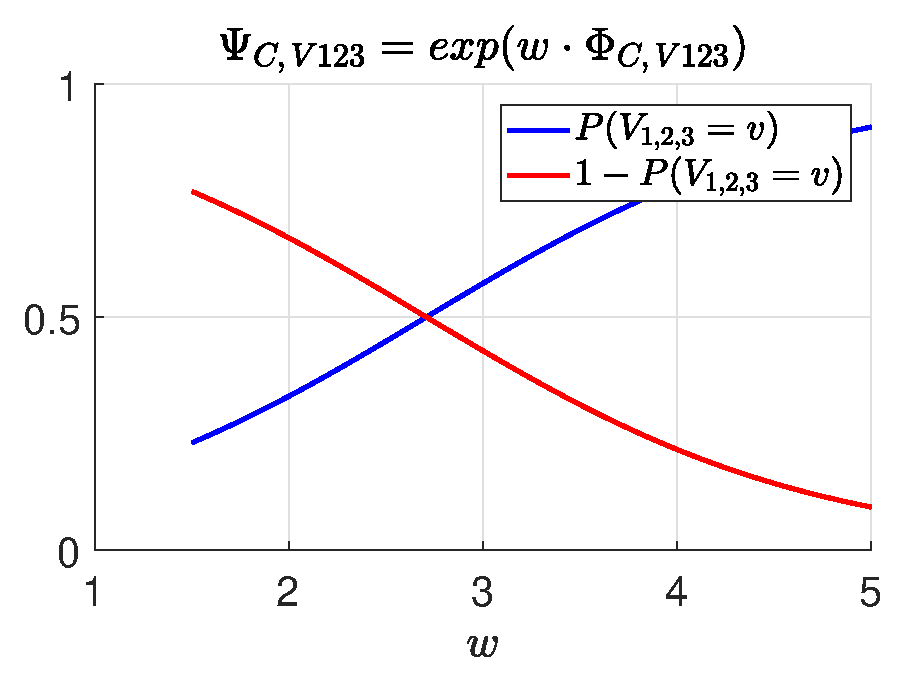
\includegraphics[width=\columnwidth]{../Chapter_additional/03_Samples/image_01/Ternary_corr.eps}
\end{minipage} 
 & 
\begin{minipage}[t]{0.48 \columnwidth}
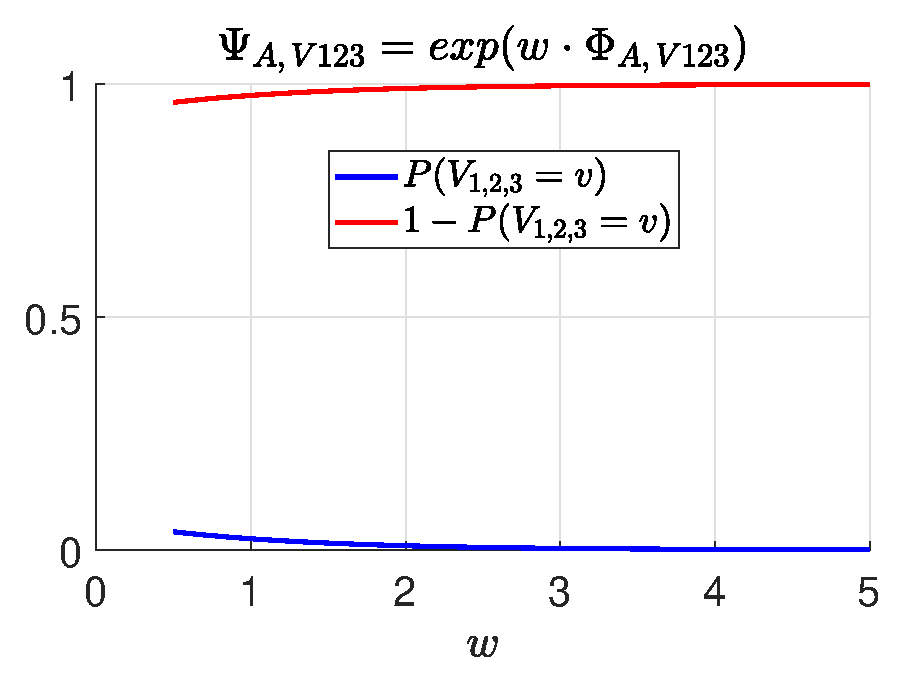
\includegraphics[width=\columnwidth]{../Chapter_additional/03_Samples/image_01/Ternary_anitcorr.eps}
\end{minipage} 
\end{tabular}
\caption{The probability $\mathbb{P}( V_1 = v,  V_2 = v, V_3 = v | w)$ and its complement, when considering a ternary correlating factor, on the left, and an anti-correlating one, on the right.}
\label{fig:sample_01:0}
\end{figure}

Part 02 considers a ternary correlating factor $\Phi_{C\,\,V123}$, involving variables $V_1$, $V_2$ and $V_3$, each having a domain size equal to 3. Ternary factors cannot be part of a graph, but it is anyway possible to build them as distribution object.
The values in the image of $\Phi_{C\,\,V123}$ are all 0, except for those combination for which $V_1,V_2$ and $V_3$ assume the same value ($0,1$ or $2$) and in such cases, the image is equal to 1.
\\
The same example builds at a second stage a ternary anti-correlating factor $\Phi_{A\,\,V123}$. The values in the image of $\Phi_{A\,\,V123}$  are all 1, except for those combination for which $V_1,V_2$ and $V_3$ assume the same value ($0,1$ or $2$) and in such cases the image is equal to 1.
\\
When considering a graph having only $\Psi_{C,\,V123} = exp( \Phi_{C\,\,V123} \cdot w)$ as a factor, the ripartition function $Z$ is equal to:
\begin{eqnarray}
Z = (4^3 - 4) + 4 \cdot exp(w)
\end{eqnarray}
The probability to have as a realization a combination with the same values is equal to:
\begin{eqnarray}
\mathbb{P}( V_1 = v,  V_2 = v, V_3 = v ) &=& \sum _{i=0}^3 \mathbb{P}( V_1 = i,  V_2 = i, V_3 = i )  \\
&=& \sum _{i=0}^3 \frac{\Psi_{C\,\,V123}(i,i,i)}{ Z} \\
&=& 4 \cdot \frac{\Psi_{C\,\,V123}(0,0,0)}{ Z} \\
&=& \frac{4 \cdot exp(w)}{(4^3 - 4) + 4 \cdot exp(w) }
\end{eqnarray}
The value assumed by $\mathbb{P}( V_1 = v,  V_2 = v, V_3 = v | w)$  is reported in Figure \ref{fig:sample_01:0}, together with the complementary probability $1 - \mathbb{P}( V_1 = v,  V_2 = v, V_3 = v | w)$.
\\
When considering a graph having only $\Psi_{A,\,V123} = exp( \Phi_{A\,\,V123} \cdot w)$ as factor, the ripartition function $Z$ is equal to:
\begin{eqnarray}
Z = (4^3 - 4) \cdot exp(w) + 4
\end{eqnarray}
The probability to have as a realization a combination with the same values is equal to:
\begin{eqnarray}
\mathbb{P}( V_1 = v,  V_2 = v, V_3 = v ) &=& \sum _{i=0}^3 \mathbb{P}( V_1 = i,  V_2 = i, V_3 = i )  \\
&=& \sum _{i=0}^3 \frac{\Psi_{A\,\,V123}(i,i,i)}{ Z} \\
&=& 4 \cdot \frac{\Psi_{A\,\,V123}(0,0,0)}{ Z} \\
&=& \frac{4}{(4^3 - 4) \cdot exp(w) + 4 }
\end{eqnarray}
The value assumed by $\mathbb{P}( V_1 = v,  V_2 = v, V_3 = v | w)$  is reported in Figure \ref{fig:sample_01:0}, together with its complement $1 - \mathbb{P}( V_1 = v,  V_2 = v, V_3 = v | w)$.
Indeed, when the variables are correlated, i.e. they share $\Psi_{C\,\,V123}$, the probability $\mathbb{P}( V_1 = v,  V_2 = v, V_3 = v | w)$ is big. Moreover, the more $w$ is high (i.e. the more the variables are correlated), the more the latter probability is big. On the opposite, when the variables are anti-correlated, the opposite situation arises. 
